%!TEX root = ../../main.tex
%----------------------------------------------------------------------------
\chapter{Mobile Robot Design}\label{chap:mobile_robot_chapter}
%----------------------------------------------------------------------------

The mobile platform performed the task of transporting the LEGO bricks between the dispenser unit, and the robot cell. It had to be able to fulfill this task in a completely autonomous manner under normal operation, avoid collision with obstacles, be harmless to its operators and be remotely controllable through a human machine interface. It was also a requirement that its progress should be monitored through the aforementioned user interface. 

Due to the high complexity of the task, we decided to pursue a modular approach. In this chapter we will introduce the components comprising the system, the motivation for having them, their implementation and the reasons behind the choices we made during the design process.



% Please keep sections separated in their designated folders and only reference them here using the input tag

%!TEX root = ../../main.tex
\section{Hardware} % (fold)
\label{sec:mr_hardware}

\textbf{Provided hardware}
\\
\\
The platform for the mobile robot revolves around the SDU FrobitPro wheeled 
robot, mounted with a tip loading platform. The whole system is driven 
by a micro-atx computer system with Ubuntu 14.04 and Ros indigo to form the 
Frobomind system. As power source is a 12V 7000mAh lead battery (same type as 
used for 
small mopeds) and a SDU Frobomind controller, that also act as a controller for 
the driving motors. To enable a continous operation of the mobile robot, an 
intelligent CTEK 5.0A charger was used. This provided enough charging 
capability to test the system for an indefinite time while connected.\\ An 
overview of the robot can be seen in Figure \ref{fig:frobit}.It was arbitrarily 
chosen that the front of the robot would be in the end with the small wheel.\\
\begin{figure}[H]
	\centering
	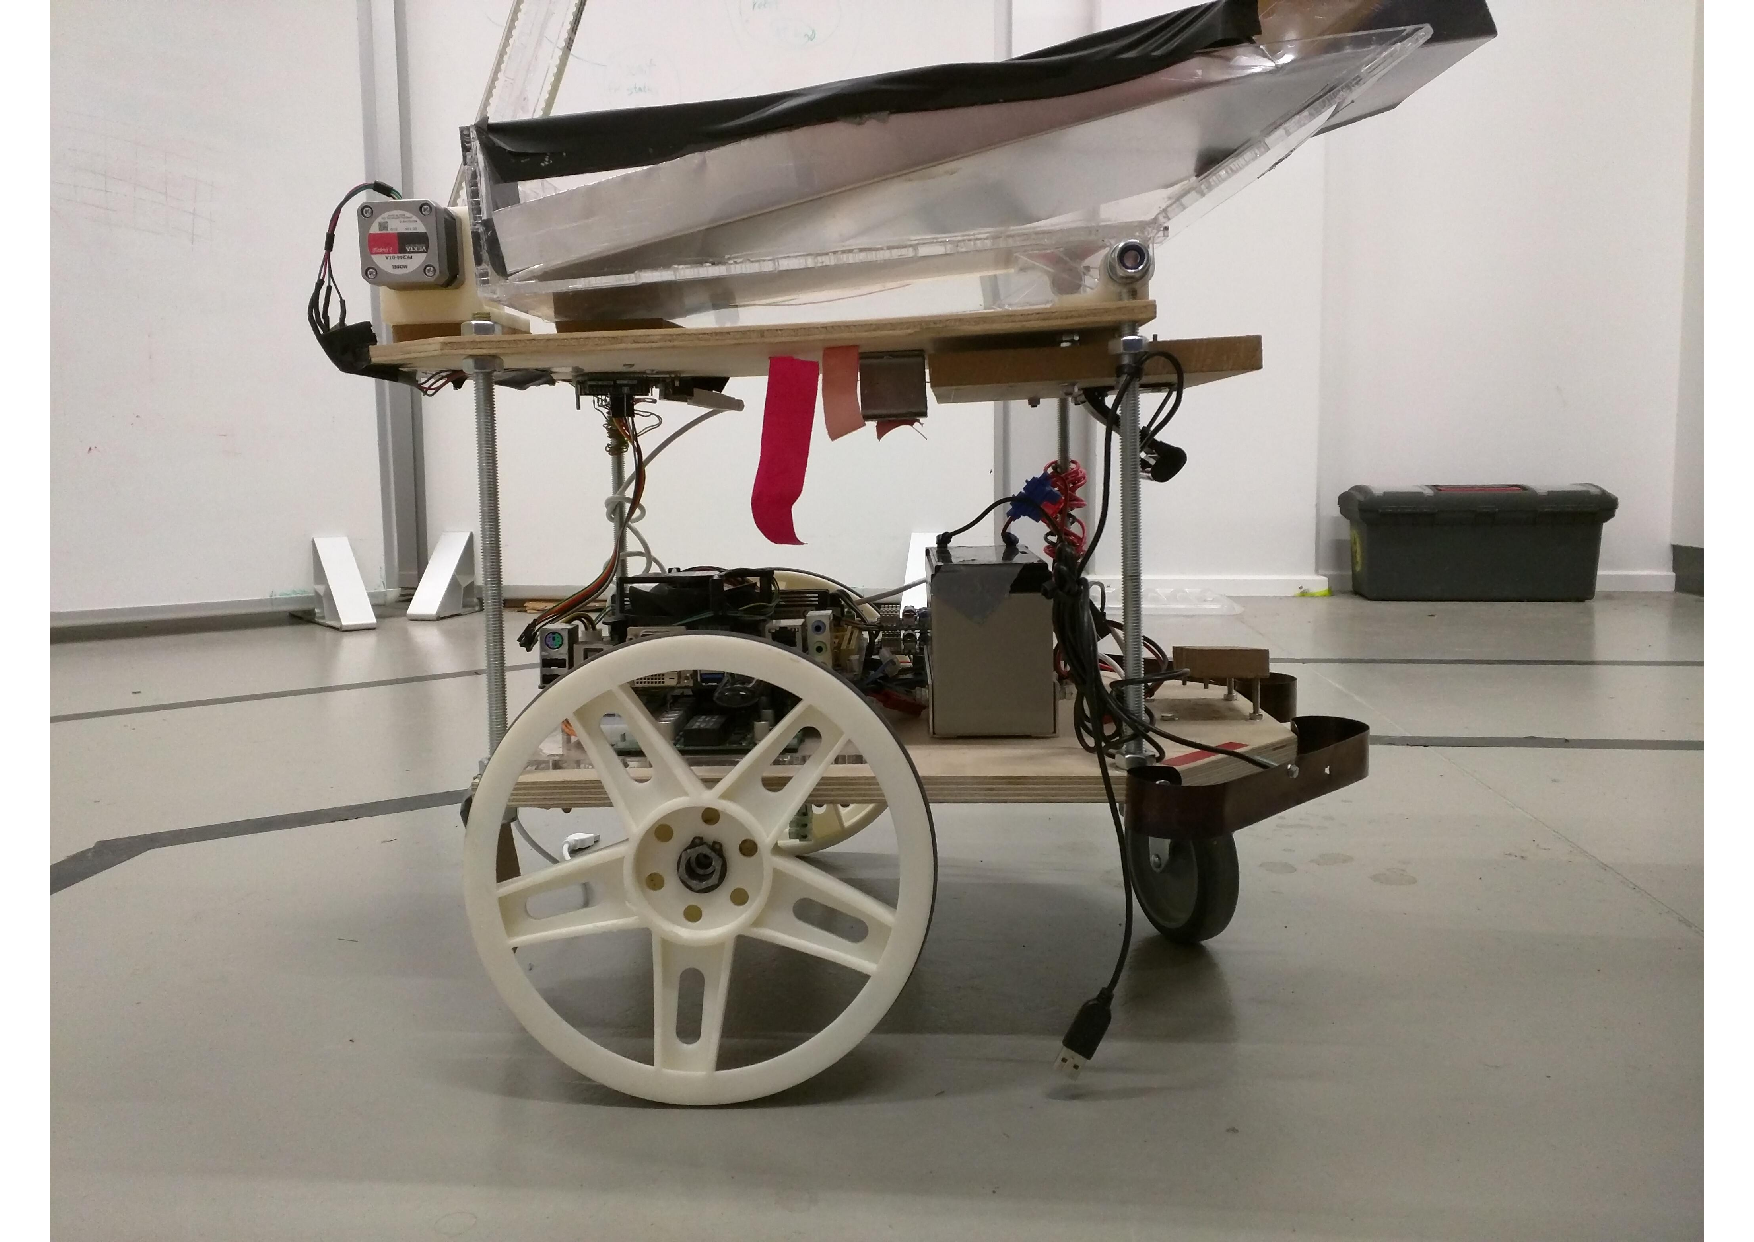
\includegraphics[width=0.7\textwidth]{frobit_profile}
	\caption{FrobitPro Robot}
	\label{fig:frobit}
	\end{figure}
\textbf{The main components for the tipper:}
\begin{itemize}
	\item PK-244-01A Bipolar Stepper motor
	\item Arduino UNO
	\item L298N dual H-bridge control board (Self-obtained)
	\item 2x Microswitch w/arm as end-point sensors for the motion
\end{itemize}   

To obtain valuable information about the surrounding environment, following 
sensors were used:
\begin{itemize}
	\item Sick LIDAR laser scanner
	\item VectorNav	 IMU
	\item Logitech Webcam
\end{itemize} 

The use of these sensors will be described in the appropriate sections. The IMU 
and LIDAR was on lend from the student library.\\
\\
\textbf{Modifications}\\
Along the development and testing phase of the project it was discovered that 
custom hardware modifications was necessary for the sensors to be mounted 
properly to the robot, in regards to protection of the sensors and be able to 
make proper use of these.\\

It was decided pre-hand that it was not allowed to make adjustments(e.g. 
cutting and drilling) in the base plate of the robot, of which it was chosen 
that the line-following camera would be mounted below the tipper without 
obstructing the LIDAR's field of view. This can be seen in figure 
\ref{fig:webcam_mr}.
\begin{figure}[H]
	\centering
	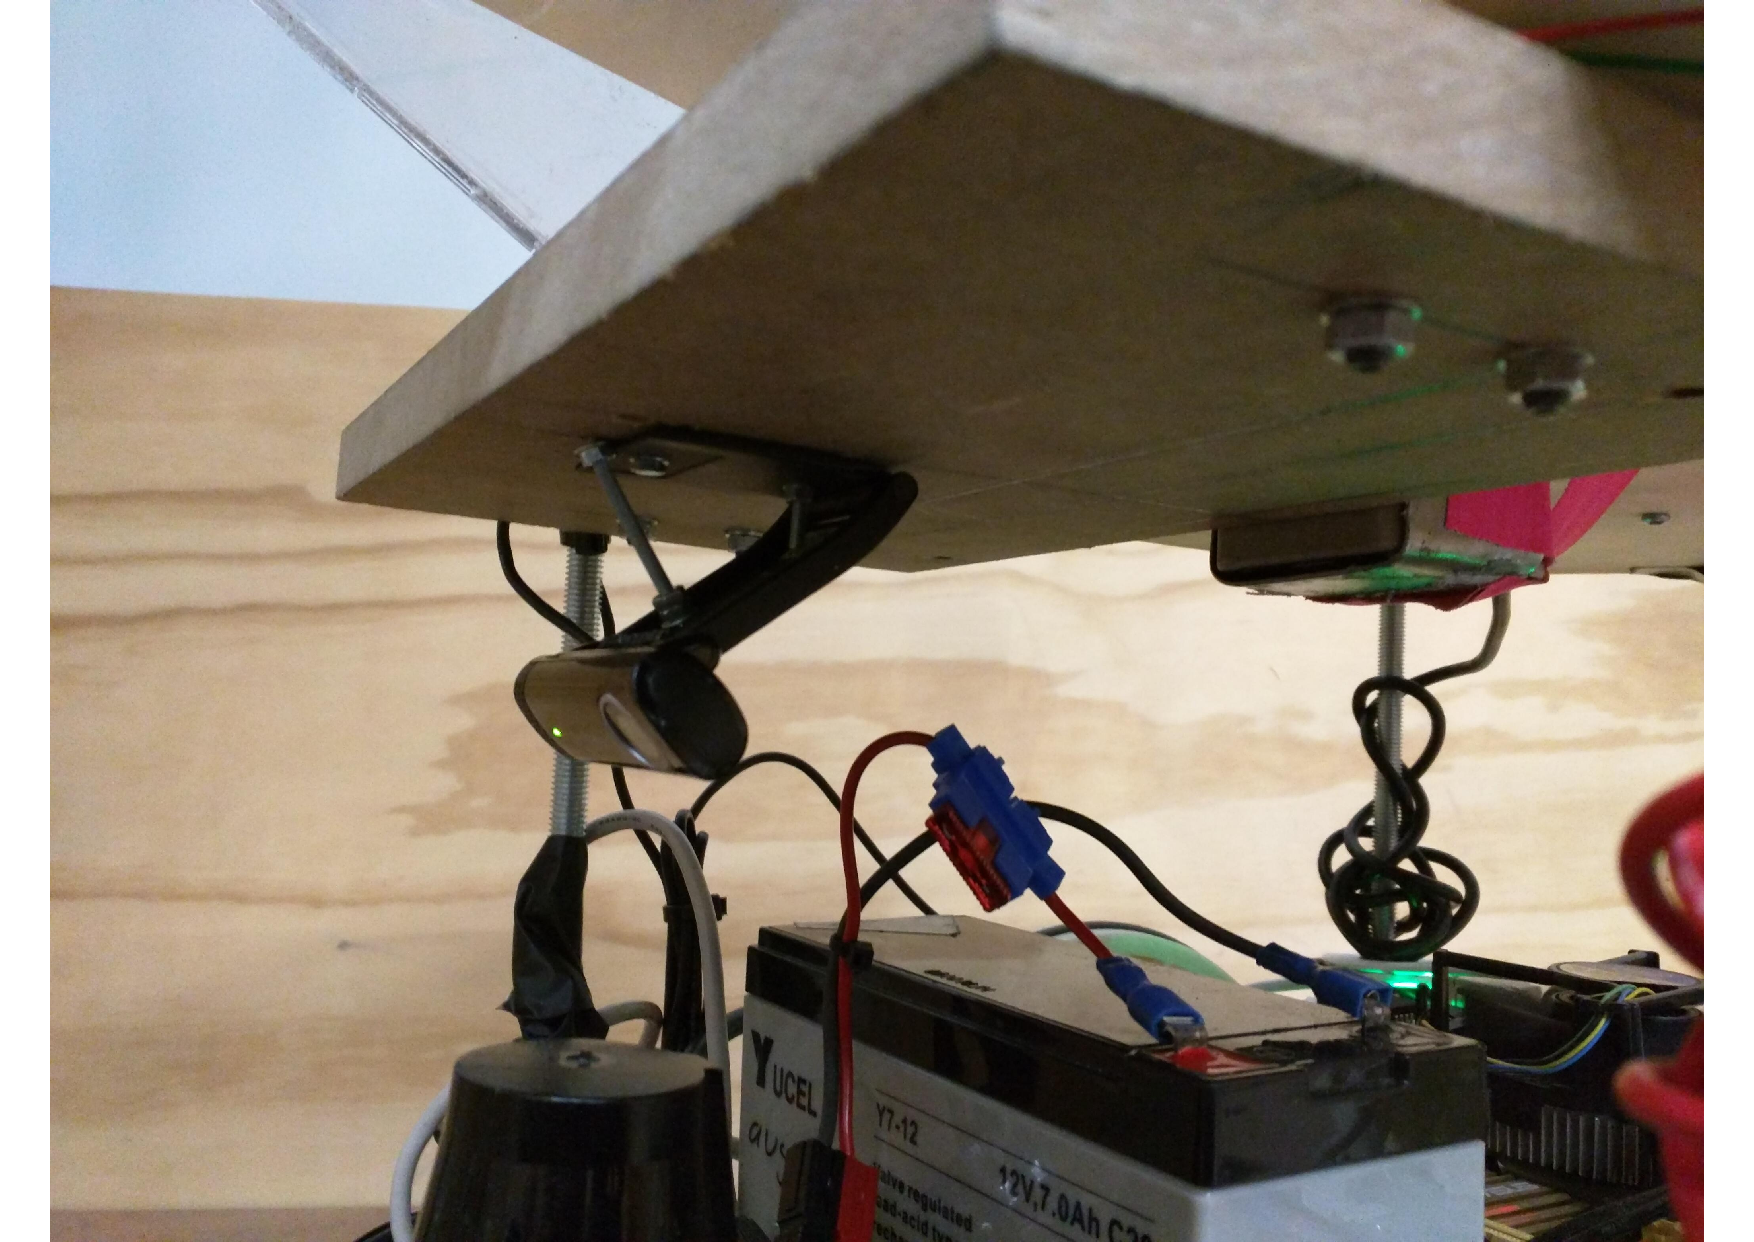
\includegraphics[width=0.7\textwidth]{webcam_mr}
	\caption{Line-following/QR detection camera}
	\label{fig:webcam_mr}
	\end{figure}
The previous use of an IMU on the robot had a remaining mount. With duct tape 
this was firmly attached. This can also be seen in figure \ref{fig:webcam_mr} 
in the background.
\begin{figure}[H]
	\centering
	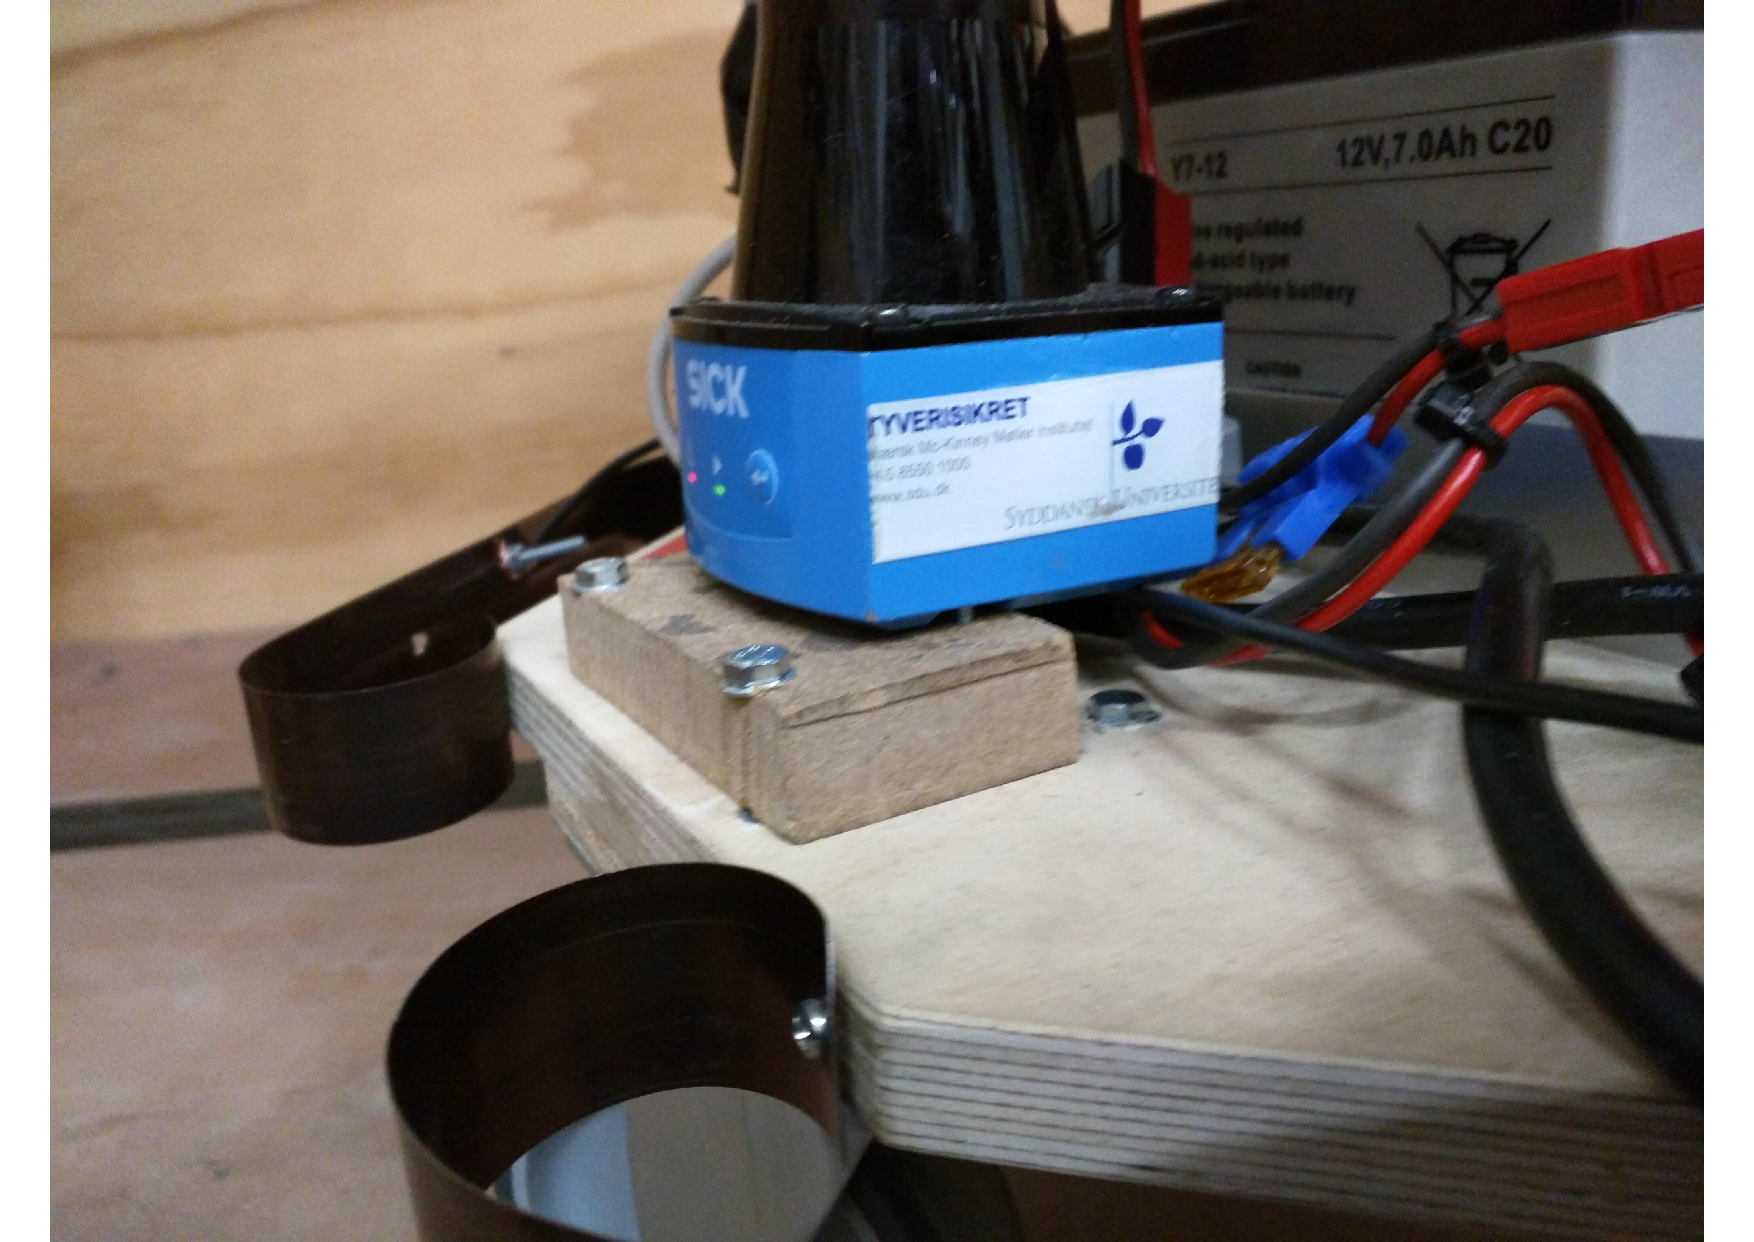
\includegraphics[width=0.7\textwidth]{lidar}
	\caption{Lidar laser scanner}
	\label{fig:lidar}
\end{figure}

In the preliminary tests, the Lidar was put on a wooden board in front of the 
robot to get as much use of the 270 degrees sensor as possible. 
Experimentally and in regards to the price of this sensor, it was later chosen 
to move it within the robot base to avoid any mishaps during an unforseen 
collision. See figure \ref{fig:lidar}. This obviously sacrifices some of the 
sensor angle.


The Arduino and H-bridge for the tipper control was mounted close to the 
stepper motor as shown in figure \ref{fig:arduino}. After some 
testing/collisions with the other robots, the usb plug of the arduino board had 
to be reattached and the board was therefore moved so nothing would interfere 
with the usb plug during runs. 

\begin{figure}[H]
	\centering
	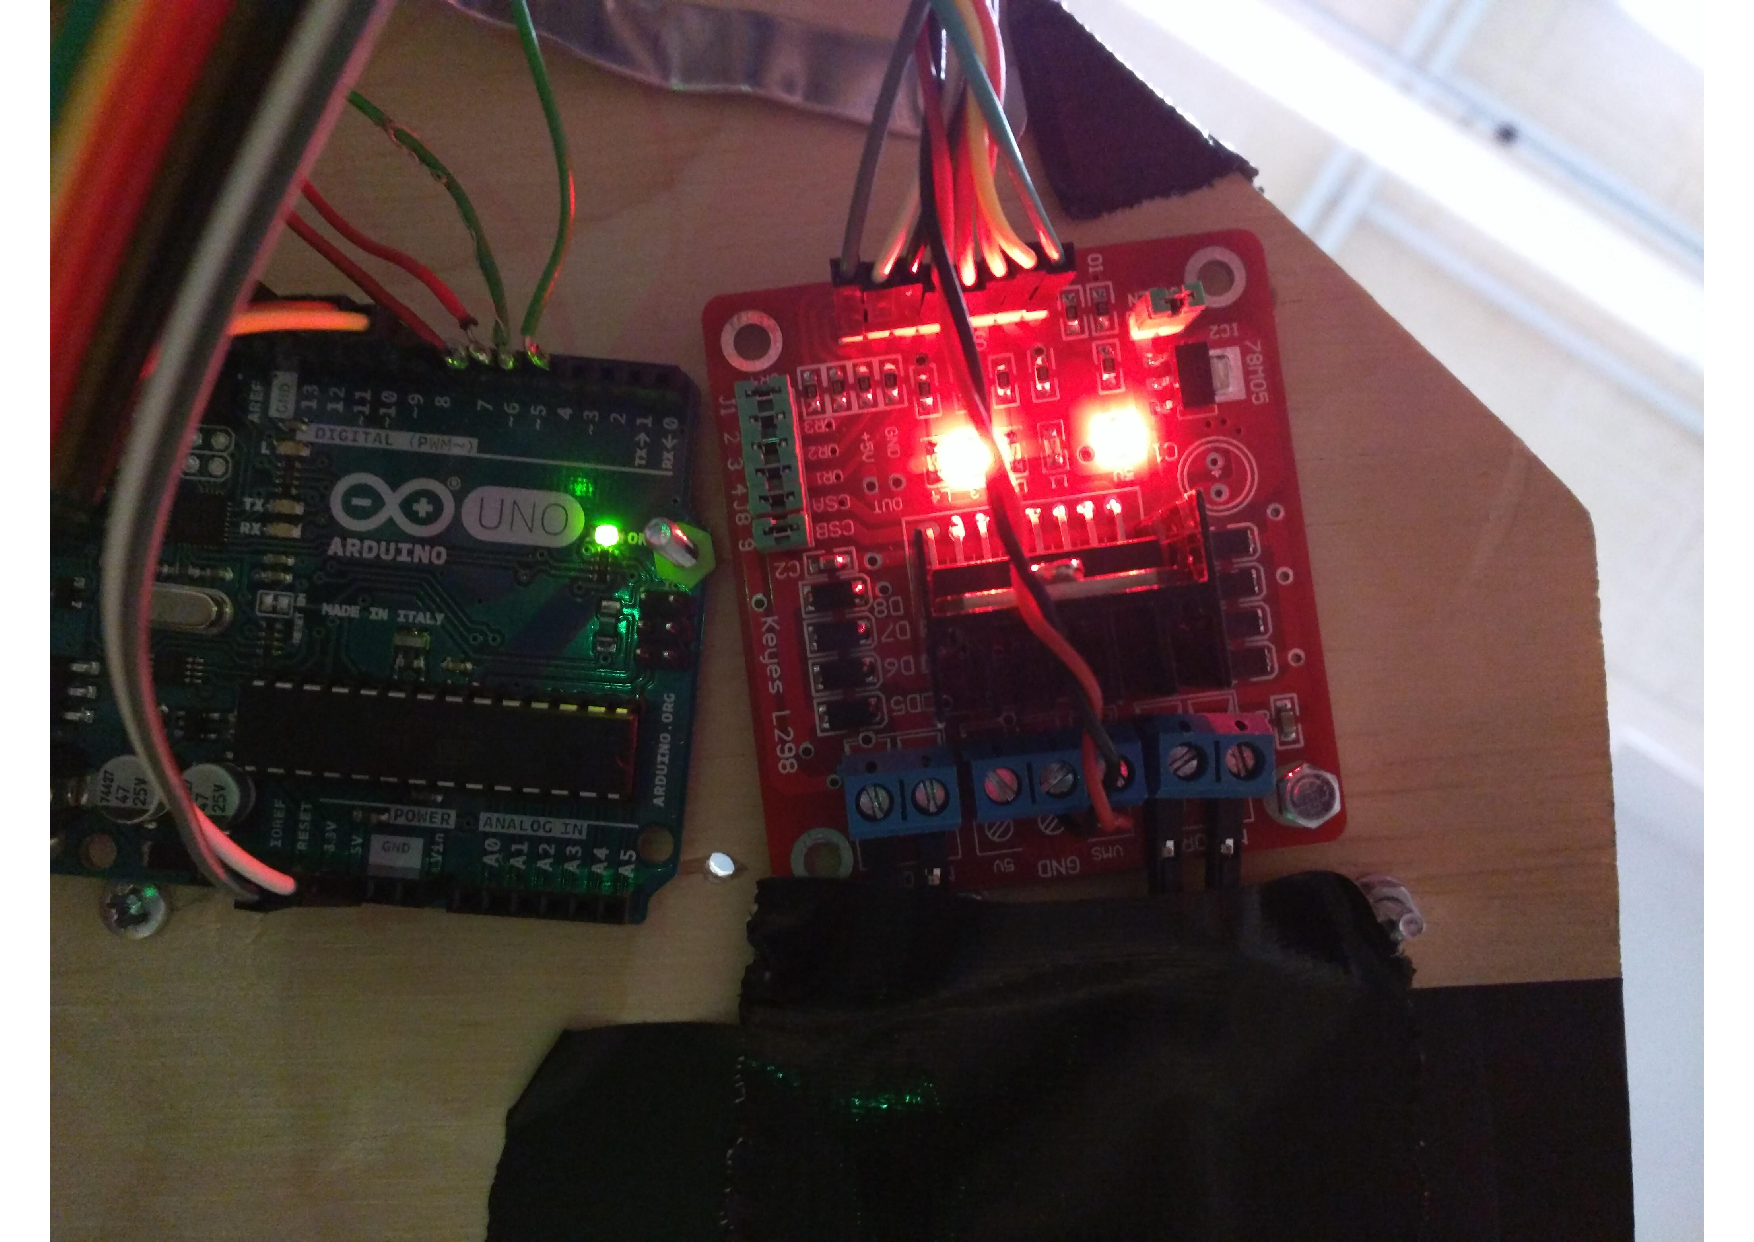
\includegraphics[width=0.7\textwidth]{arduinoandhbridge}
	\caption{Arduino and H-bridge mounted on the robot}
	\label{fig:arduino}
\end{figure}

During docking sessions in the dispenser/charging station, it was discovered 
that attaching a bumper-like system would increase the angle of which the robot 
could enter the charging station thus reducing the strictness of localization 
for going to the charger. The bumper idea can be seen in 
\ref{fig:bumper}.  


\begin{figure}[H]
	\centering
	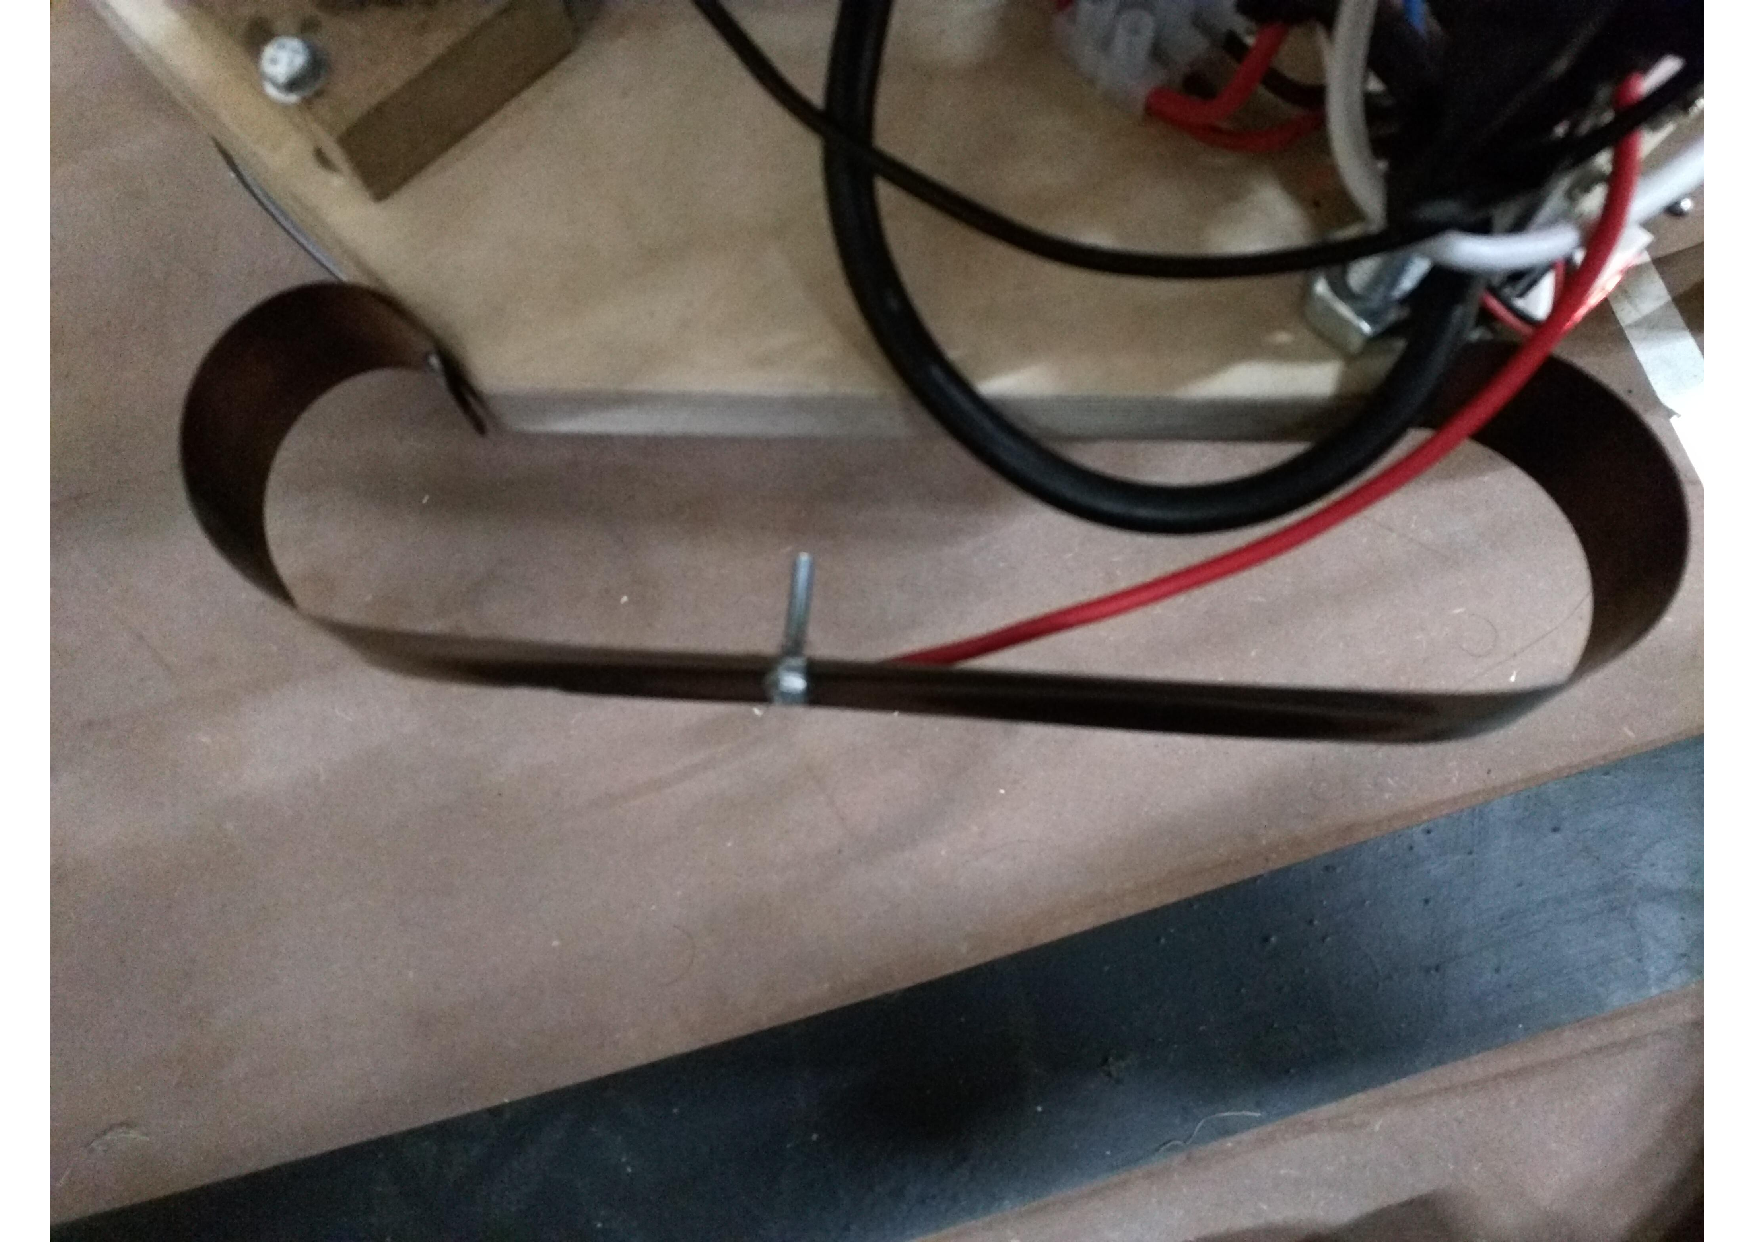
\includegraphics[width=0.7\textwidth]{bumper_mr}
	\caption{Bumper on the Mobile robot}
	\label{fig:bumper}
\end{figure}
Finally the plexiglas tray on top of the robot was found inadequate to deliver 
all bricks at the conveyor belt, so an aluminium insert was created. To ensure 
that the bricks were delivered to the conveyor belt and not next to it, this 
insert was created with a narrow tip, as seen in \ref{fig:tray}

\begin{figure}[H]
	\centering
	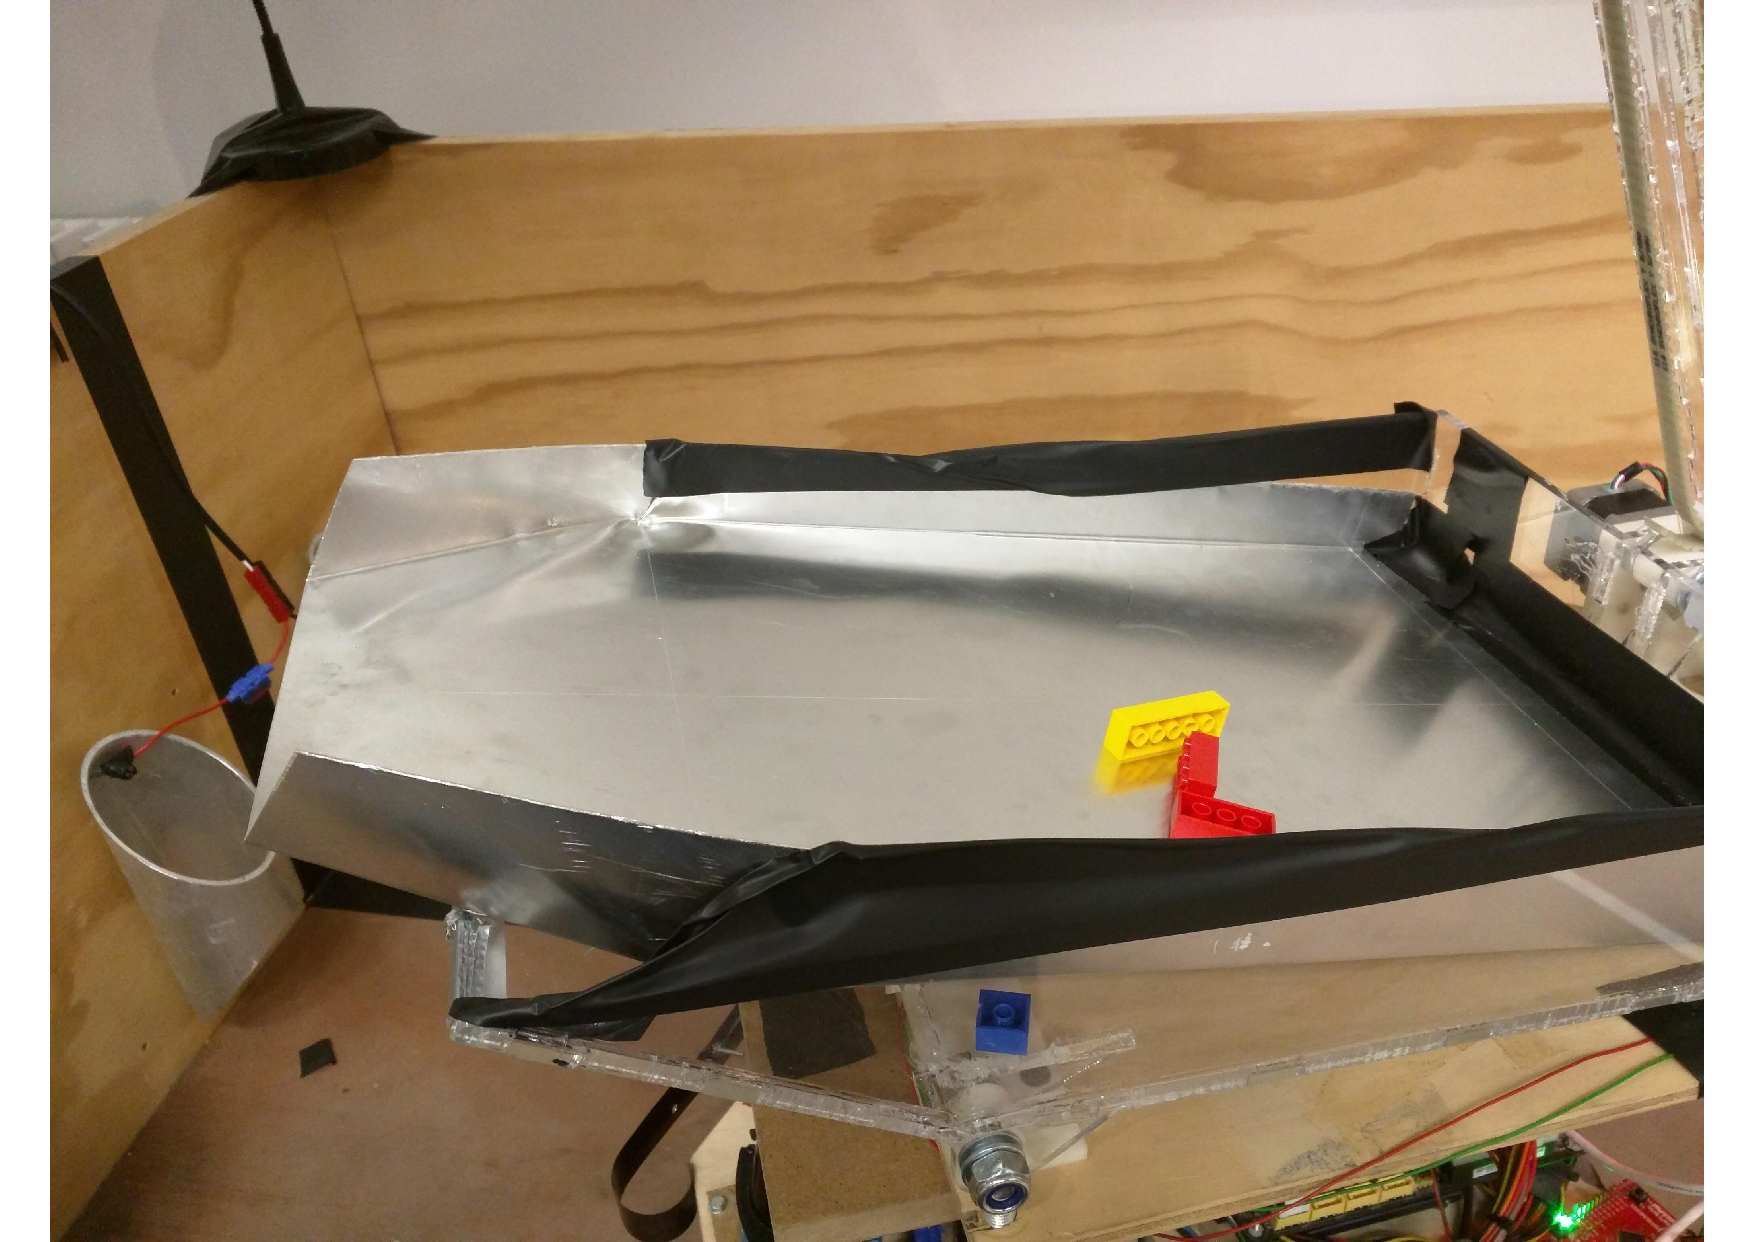
\includegraphics[width=0.7\textwidth]{trayside}
	\caption{Aluminium tray insert on the mobile robot}
	\label{fig:tray}
\end{figure}

% section hardware (end)
%!TEX root = ../../../main.tex
\section{Frobomind} % (fold)
\label{sec:mr_frobomind}

\textbf{Someone}

A shord tesciptiotion of FroboMind, what it is, the benefit of using it in comparison to a purely ROS based system, and how we use it now...

	\subsection{Frobomind interface} % (fold)
	\label{sub:mr_frobomind_interface}
	The frobomind interface is in charge of transform the hardware sensors values into ROS messages that can be used by the user.
	This is implemented as a ROS package given inside of the frobomind framework.
	A small modification in this package has been made so the status of the battery can be read.
	This allows the robot to create subrutines of charging when needed and continuing with the previous task when charged.
	% subsection frobomind_interface (end)
% section frobomind (end)


%!TEX root = ../../../main.tex
\section{Flow control overview} % (fold)
\label{sec:mr_flow_control_overview}
As explained in the chapter \ref{chap:mes_server_chapter}, the MES server sends an order and the clients have to read it and act consequently.
In the case of the mobile robot, there is a node in charge of do all the necessary steps in order to complete the order.

The flow control of the mobile robot is depicted in the figure \ref{fig:flow_control}.
This is:
\begin{enumerate}
	\item Wait for an order from the MES server.
	\item Read the order and go the brick dispenser to get some bricks.
	\item Go the the conveyor stated in the order.
	\item Tell to the MES server to activate the conveyor and unload the bricks previously picked up.
	\item Go to the position in which the robot of the workcell leave the order.
	\item Wait for the robotic arm to finish the order.
	\item Go to charge.
\end{enumerate}

\begin{figure}[htb]
	\centering
	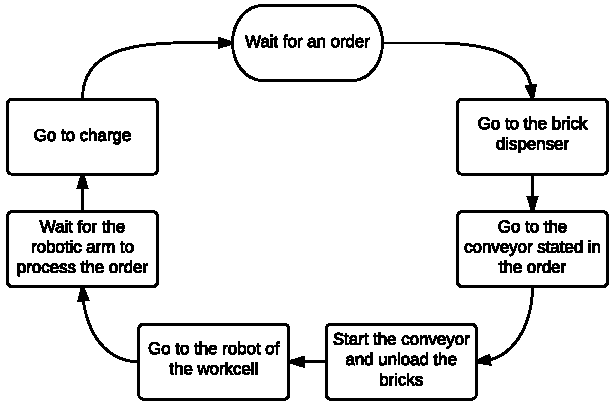
\includegraphics[width=0.75\textwidth]{flow_control}
	\caption{Flow control of the main node in the mobile robot}
	\label{fig:flow_control}
\end{figure}

This process is handled by the \emph{main node}, and this is the highest abstraction level in the control of the robot.
It is responsible of coordinate and actuate a second layer of abstraction which, at the same time, will be responsible of directly actuate the hardware.
The communications between the \emph{main node} an the second layer of abstraction, is shown in the figure \ref{fig:main_connections}.

\begin{figure}[htb]
	\centering
	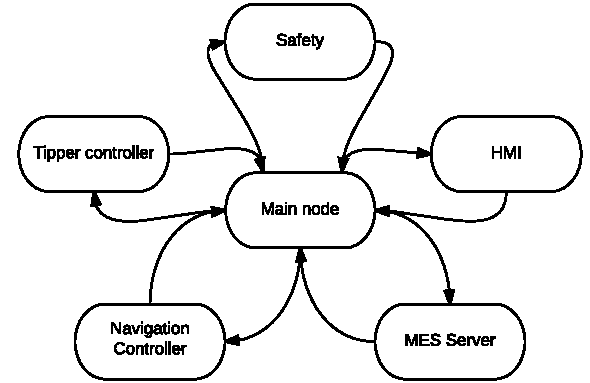
\includegraphics[width=.75\textwidth]{main_connections}
	\caption{Connections of the main node}
	\label{fig:main_connections}
\end{figure}

The main node has also an internal state of the robot represented in three states: \emph{idle}, \emph{auto} and \emph{manual}. 
The mode \emph{idle} means that the robot is not moving or executing any action. 
The mode \emph{auto} means that is processing an order and, consequently, it can be moving. \emph{Manual} stands for when the robot is being moved manually with the HMI. 
The states are intrinsically exclusive and the robot can only be controller manually if the robot is not processing an order.
This avoids the possibility of the user to interfere in the order status increasing the stability and reliability.

The connections are bidirectional and their functions are:
\begin{enumerate}
	\item \textbf{Safety}: Reads the state of the different sensors in the robot that measure the possibility of harm the robot and, if in danger, sends a signal to stops all the actuators.  
	\item \textbf{HMI}: This can change the state of the robot to \emph{auto} to start/continue an order, to \emph{idle} to pause the current order or to \emph{manual} if the user wants to control the robot manually. On the other hand, the main node can tell the HMI (1) its position and (2) the actions being carried out in that moment. This is that in the HMI is shown if the robot is, for example, inside the box and following the line or doing a relative movement.
	\item \textbf{MES server}: The main node reads the order sent and starts the new hierarchy of actions. Also the main node can send messages to the MES in order to activate other agents controlled by this.
	\item \textbf{Navigation controller}: As will be explained in the sections \ref{sec:mr_navigation_controller}, it is responsible of, knowing the current position of the robot, calculate a path to the desired position and perform it. The main node can receive from it when the robot has reached the desired position.
	\item \textbf{Tipper controller}: Handles the position of the tipper assembled in the robot. The controller can talk to the main node to tell when has finished the desired movement.
\end{enumerate}

% section flow_control_overview (end)


%!TEX root = ../../../main.tex
\section{Sensors and data processing} % (fold)
\label{sec:mr_sensors_and_data_processing}

	\subsection{Camera processing} % (fold)
	\label{sub:mr_camera_processing}
	

	\begin{figure}
        \centering
        \begin{subfigure}[ht!]{0.296\textwidth}
            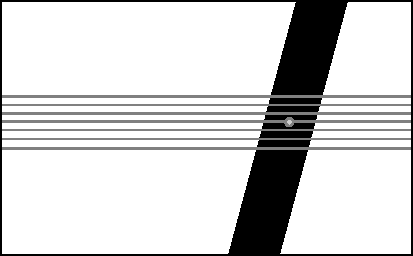
\includegraphics[width=\textwidth]{figs/mr_camera_processing_1}
            \caption{Clear detection of the line}
            \label{fig:mr_camera_processing_1}
        \end{subfigure}
        \hspace{40pt}
        \begin{subfigure}[ht!]{0.296\textwidth}
            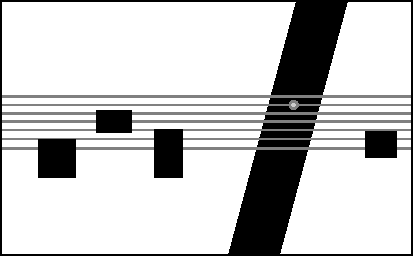
\includegraphics[width=\textwidth]{figs/mr_camera_processing_2}
            \caption{Detection when noise in the image}
            \label{fig:mr_camera_processing_2}
    	\end{subfigure}
    	\begin{subfigure}[ht!]{0.296\textwidth}
            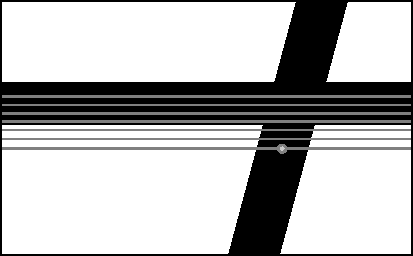
\includegraphics[width=\textwidth]{figs/mr_camera_processing_3}
            \caption{Detection when crossing line}
            \label{fig:mr_camera_processing_3}
    	\end{subfigure}
    \caption{Representation of possible cases when detecting the line}
    \end{figure}

	% subsection camera_processing (end)

	\subsection{Lidar processing} % (fold)
	\label{sub:mr_lidar_processing}
	
	% subsection lidar_processing (end)

	\subsection{Combined frobit odometry} % (fold)
	\label{sub:mr_combined_frobit_odometry}
	Wheels + IMU
	
	% subsection combined_frobit_odometry (end)

% section sensors_and_data_processing (end)
%!TEX root = ../../../main.tex
%%---------------------------------------------------------------------------
\section{Mobile Robot Navigation \label{sec:navigation_sec}}
%%---------------------------------------------------------------------------

How the mobile robot navigates in general (system overview), and the discussion of its subsystems in details (why, how, how well):
\begin{itemize}
    \item Navigation Controller
    \item In-box navigation
    \item Out-of-box navigation
    \item Line following
    \item QR-code reading
    \item HMI
\end{itemize}
\subsection{In-box Navigation} \label{sec:in_box_navigation}
As per project description, the navigation inside the box is to be done based on SLAM. Due to complexity of the entire project and potential diversity of SLAM implementations, an open-source implementation of SLAM was chosen. More specifically the gmapping-package \cite{gmapping} which has a livid community of supporters and builds a ROS wrapper for “OpenSlam's Gmapping”\cite{openslam}. TF-Frames of Lidar, IMU and the robot base were set up, this allows for easy transformation between Lidar and odometry data, inside the package. Using these, the SLAM-Implementation uses a particle filter to sequentially build up a map of the area. By manually driving through the entire workspace, a map was created. 
\begin{figure}[H]
	\centering
	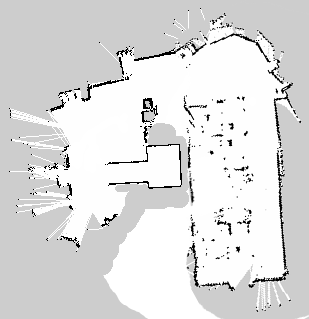
\includegraphics[width=0.5\textwidth]{slam_map}
	\caption{Slam Map}
	\label{fig:slam_map}
\end{figure}
Using the map-server package from the ROS 2D-Navigation Stack \cite{navigation_stack} the generated map was stored and is then broadcasted as a static map for localization. The AMCL (Adaptive Monte-Carlo Localization) package (which is also included in the navigation stack) then uses the static map, the lidar as well as odometry data to localize the robot while in free navigation. After tuning the parameters, AMCL worked fairly reliably for navigation both inside and outside the box.\\
\textbf{TODO: Describe move{\_}base}\\
Due to the box being fairly monotone in respect to the Lidar readings (clean, walls, no landmarks), precise navigation inside the box was sometimes not perfect. Also with multiple robots present in the box, issues, especially when trying to charge occurred. To ensure reliability of charging, a backup behaviour was added, when the charging failed using move{\_}base. For this a line was added, using the already implemented Line Following behaviour. The move{\_}base is used to navigate the robot to the start of the charging line. Then the robot follows the line until a pre-specified distance from the wall using Lidar. Having a main and a backup behaviour proved to be sufficient for reliable charging\\
\textbf{TODO: IS THAT REALLY SO?}
%!TEX root = ../../../main.tex
\section{Tip controller} % (fold)
\label{sec:mr_tip_controller}

The purpose of tip controller is to create a simple and effective way of 
delivering a large amount of LEGO bricks to the conveyor belt autonomously. 
This is done by controlling the mounted belt drive with a stepper motor, an 
H-bridge and a Arduino microcontroller. To control the limits of tipping 
mechanism, two microswitches were added(Tip down/tip up).\\

\subsection{Stepper controller} % (fold)
\label{sub:stepper_controller}
The PK-244-01A stepper motor is bipolar. This means that it requires (at least) 
four wires to control the two coils in contrast to a unipolar motor which has 1 
supply wire and usually only requires two control wires. 
The four wires are driven by the L298N dual 
H-bridge, powered by 12V from on-board pc power supply. Four control pins are 
connected to the 
Arduino and signals on these controls the motor wires. Consulting datasheet for 
the motor, a minimum of 4V, 1.2A is required to drive the motor. Timing is 
calculated as a minimum of 
3ms delay between steps in the timing diagram. To get an initial high torque 
from the motor, a half-stepping sequence was chosen and a ramp function was 
created to slowly start the motor and exponentially increase speed when the 
tip is in full motion. Due to friction in the system and less torque the 
full-step sequence was disregarded. The Arduino software has a built-in library 
for stepper motors, but this was found difficult to manage in regards to delay 
of the steps. 
% subsection stepper_controller (end)

\subsection{Arduino and serial communication} % (fold)
\label{sub:arduino_and_serial_communication}
Setting a general serial communication to the Arduino is straight-forward. The 
speed is chosen with regards to the ROS node and a serial connection is 
initialized with the \textbf{Serial.begin(speed)} command. The Arduino is set 
up to 
receive a character "u" for tipping(up), and "d" for leveling(down). When an 
action has successfully executed, a "d" (done) is returned to the ROS node.
% subsection arduino_and_serial_communication (end)


% section tip_controller (end)

%!TEX root = ../../../main.tex
\section{Safety system} % (fold)
\label{sec:mr_safety_system}
The safety in the mobile robot is intrinsic in all the nodes that allow its movement.
Additionally the Safety Eyes was supposed to be used to detect humans in the area close to the stairs. However due it not working, it was not being used.
There then are two aspects to talk about: (1) the \textbf{incident handler} based on the the given frobomind implementation. Based on certain inputs, an \emph{activation} signal is created, allowing the robot to move.
(2) On the other hand, the \textbf{obstacle detector} is used to feed another skill (see section \ref{sub:skills}) that changes the speed, or even stops, the robot depending on the distance of obstacles detected by the LIDAR.
This can be activated or disabled depending on the situation.
	\subsection{Incident handler} % (fold)
	\label{sub:mr_incident_handler}
	The incident handler is based in the \emph{simple incident handler} given inside of the frobomind framework.
	This system receives two signals: (1) the \emph{deadman} and (2) the \emph{critical fault}.
	When both signals are received correctly, the incident handler outputs another signal that \emph{enables the actuation}.
	This signal is directly received from the system that actually performs the actions that move the motors in the robot.
	Both signals are booleans with a time stamp and need two conditions to be approved:
	\begin{enumerate}
		\item As booleans, need to be true.
		\item As stamped, need to be received in an interval smaller than a threshold. In our system the signal need to be received in intervals inferior to 50 milliseconds.
	\end{enumerate}
	If both, \emph{deadman} and \emph{critical fault}, are received by the incident handler satisfying those conditions, the output signal \emph{actuation enable} will be published and the robot will move.
		\subsubsection{Deadman} % (fold)
		\label{ssub:mr_deadman}
		The deadman signal is used by the navigators to actually perform a movement.
		As stated previously, the signal needs to be sent in intervals lower to 50 milliseconds and be true.
		The deadman signal received in the incident handler doesn't contain information about who is the sender, but is not a problem due to the navigators are made so they are exclusive.
		This means, that only one deadman signal is received from one navigator.
		% subsubsection deadman (end)

		\subsubsection{Critical fault} % (fold)
		\label{ssub:mr_critical_fault}
		The critical fault signal is controlled by the main controller of the robot.
		This node, as explained in the section \ref{sec:mr_flow_control_overview}, controls among others the mode of the robot.
		Only in the modes \emph{manual} and \emph{auto} this signal is activated meaning that if the robot is in \emph{idle}, either because there was a critical fault in the robot or because manually was stopped, the robot cannot move.
		As stated previously, the signal needs to be sent in intervals lower to 50 milliseconds and be true.
		% subsubsection critical_fault (end)
	% subsection incident_handler (end)

	\subsection{Obstacle detector} % (fold)
	\label{sub:mr_obstacle_detector}
	Its function consist of reading all the distances information from the LIDAR and, given a detection angle and two thresholds (\emph{proximity alert} and \emph{colliding}), output a signal which will slow down or stop the robot.
	The obstacle detector is used inside of an skill (see section \ref{sub:skills}) so it can be activated or disabled when necessary.

	In practice the obstacle detector is only used in places where (1) there is a risk to crash and (2) its behavior doesn't affect to the main one.
	This means that, for example, inside of the robotic arm workcell it is disabled due to (1) the robot cannot crash with any moving agent and (2) due to the proximity to other static parts inside the workcell, it would be in the \emph{proximity alert} mode all the time. 

	% subsection obstacle_detector (end)

	The output of the obstacle detector can be three different exclusive states: (1) \emph{safe}, (2) \emph{proximity alert} and (3) \emph{colliding}. 
	The default mode is \emph{safe}, while the other two modes are enabled based on two thresholds.
	The thresholds are expressed in the same units as the distance received from the LIDAR being in our project 40 cm for \emph{proximity alert} and 15 cm for \emph{colliding}.
	When in \emph{proximity alert} the robot will slow down its movement (any) in a factor of 0.5 and when in \emph{colliding} will stop.

	The limitations of this system is that with the LIDAR being mounted in the front, only obstacles which are in the area of the LIDAR can be detected.
	So no obstacles in the sides and behind are detected and these movements are "blind".
% section safety_system (end)

%!TEX root = ../../../main.tex
\section{Human Machine Interface} % (fold)
\label{sec:mr_human_machine_interface}

Motivation for having one, capabilities, implementation, testing and results.

	\subsection{Web} % (fold)
	\label{sub:mr_web}

	% subsection web (end)

	\subsection{Physical devices} % (fold)
	\label{sub:mr_physical_devices}
	Talk here about the button too.

	% subsection physical_devices (end)

	\subsection{ROS Services} % (fold)
	\label{sub:mr_ros_services}

	% subsection ros_services (end)

% section human_machine_interface (end)
